\section{Renderer Communication}
\label{chapter:implementation:renderer}

	\begin{figure}[htbp]
		\centering
		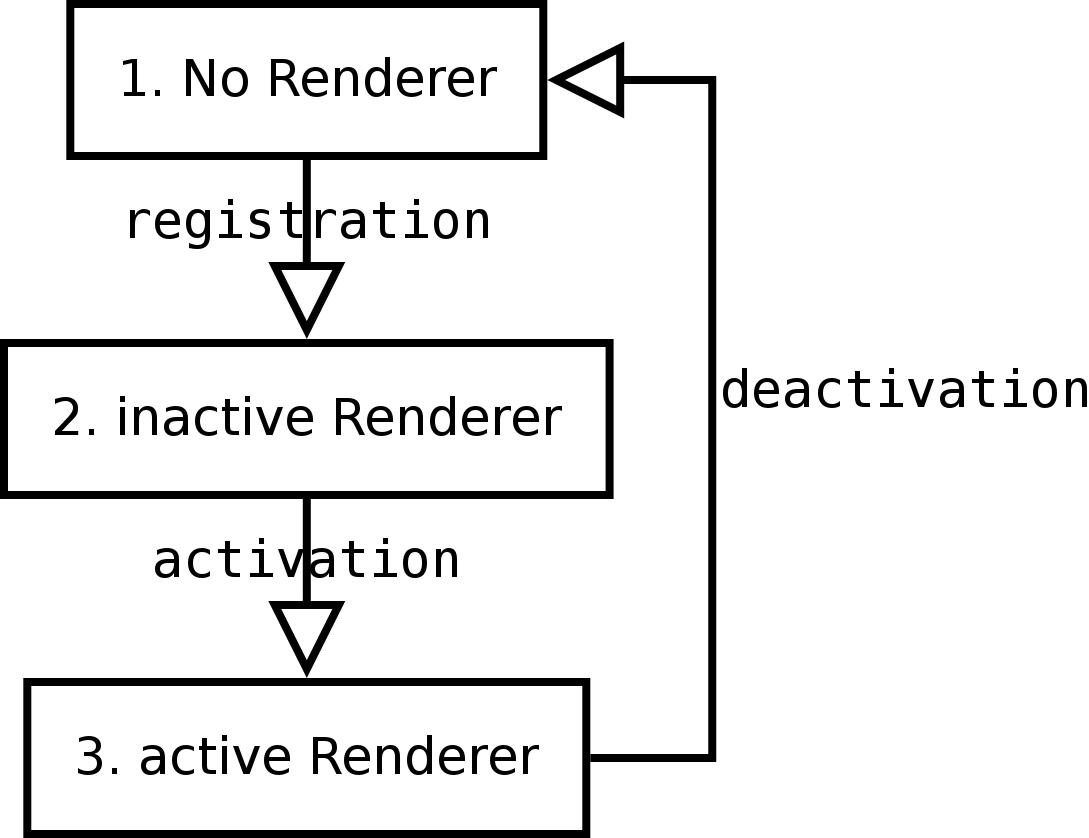
\includegraphics[width=6cm]{images/RendererFlowchart.png}
		\caption{All states and some possible state changes regarding the external renderer.}
		\label{fig:RendererFlowchart}
	\end{figure}

	\clubpenalty=10000
	\widowpenalty=10000

	The external renderer is implemented as a replaceable component of the library. Because of this approach, the communication between this component and the rest of the library needs to be divided into several states, depending on the presence of the renderer and whether it is active or not. The flowchart in figure \ref{fig:RendererFlowchart} shows the state changes between

	\clubpenalty=150
	\widowpenalty=150

	\begin{numlist}
		\item the initial state of the library without any registered renderers,
		\item the operation with an inactive renderer and
		\item the state an application usually runs in -- where the output of the scene is being rendered.
	\end{numlist}

	The flow of information between PURGE and its rendering component was defined as follows:

	\begin{smalllist}
		\item No registered renderer: All operations on objects are performed within PURGE, any parameter changes are stored in the main library. This state guarantees that the API is capable of processing all commands independently of any implementing renderers.
		\item As soon as a renderer has been defined, it is registered as an available component in PURGE, but there is still no flow of information between the two layers.
		\item The activation of the renderer causes the first flow of data. The renderer itself will first call its own initialization routines, acquire the resources it needs, and will then receive the data forming the current scene. When this process is finished, the renderer will be called regularly by the main loop to render the scene.
		\item Once the renderer is de-activated, the renderer is expected to free all resources in order to allow another renderer to be activated -- which will possibly require some resources this renderer was holding.
	\end{smalllist}

	As outlined in the description of the state changes, there are two instants at run-time that require passing scene data from PURGE to the renderer:

	\begin{numlist}
		\item The activation of the renderer and
		\item the rendering process, which will periodically need access to the scene data in order to render it.
	\end{numlist}

	The first instance requires the transmission of all data that was generated in the absence of the renderer. The second state, however, requires merely the transmission of changes -- re-evaluating every existing object in the renderer would have an easily avoidable performance impact.

	A possible implementation could consist of a list of operations that were performed on the scene objects, which can be flushed to the renderer in both cases. This approach supports the equal treatment of both scenarios: In the first case, all operations are transmitted to the renderer, in the second case only those that have been triggered since the last transmission.

	This solution requires the tracking of any changes to the scene, which will be flushed to the renderer before the actual rendering is performed. Unfortunately, this necessity requires further optimizations to eliminate the increasing memory consumption throughout the lifetime of the application.

	The next approach is a variation on the first. Several distinct events have been defined that can be consumed by the renderer. At each cycle, the following operations are accumulated:

	\begin{smalllist}
		\item newly created objects,
		\item updated objects and
		\item destroyed objects.
	\end{smalllist}
	
	The renderer is expected to process these lists of events to implement the specified scenario. PURGE, on the other hand, is responsible for the proper accounting: Each object is present in at most one list, which ensures that

	\begin{smalllist}
		\item objects that were destroyed in the same cycle are not present in any of these lists.
		\item newly created objects are not present in the list of updated objects, even if any modifying operations were performed after their creation.
		\item destroyed objects do not appear in any other registers.
		\item objects that were not modified at all during the current cycle are not present anywhere.
	\end{smalllist}

	Updated objects further keep a list of properties that were updated during the cycle. The new values of these properties can be queried by the renderer as needed. Changing the color of a \classname{SpotLight} thus leads to the following operations within the render cycle:

	\begin{numlist}
		\item The object is marked as changed -- it is added to the list of updated \classname{SpotLight} objects.
		\item The value \inlinecode{SpotLight::CHANGE\_COLOR} is pushed onto the vector of changes of the same object.
		\item When the renderer is instructed to perform the rendering, all updated SpotLight objects are collected via \inlinecode{SpotLight::getUpdatedInstances()}, the changes to the object are retrieved and the color value of the renderer's internal \classname{Light} object is replaced by the new value retrieved by \inlinecode{purgeSpotLight->getColor()}.
	\end{numlist}

	\begin{figure}[htbp]
		\centering
		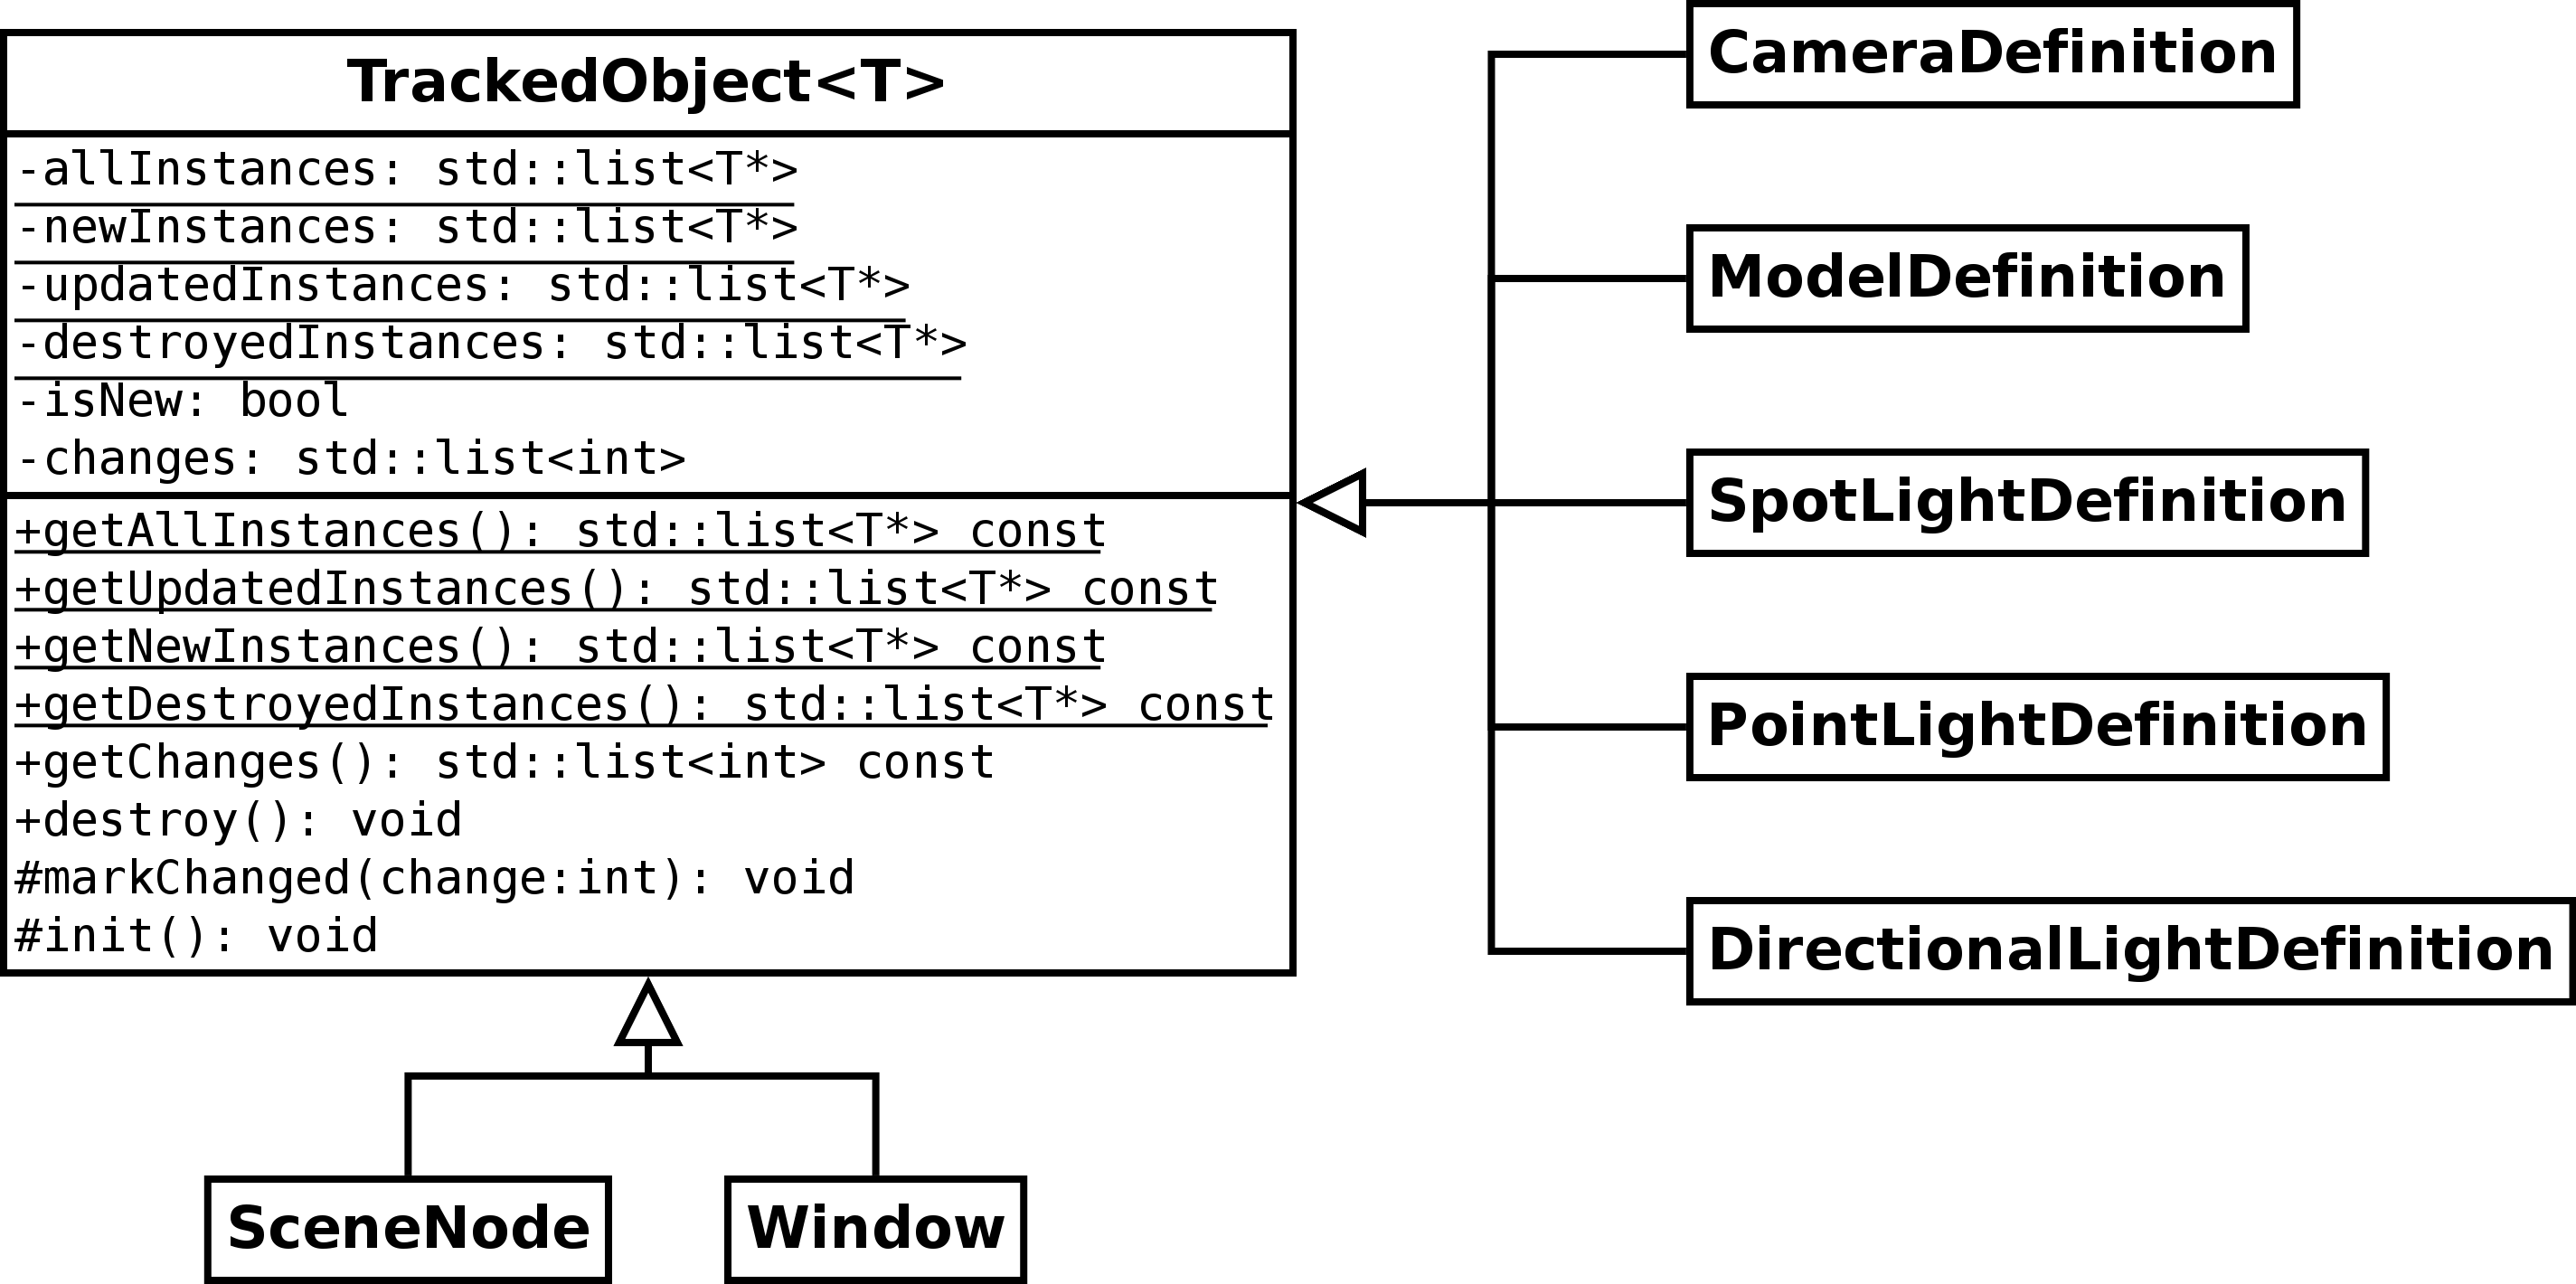
\includegraphics[width=14cm]{images/TrackedObject.png}
		\caption{Outline of the \classname{TrackedObject} class.}
		\label{fig:TrackedObject}
	\end{figure}

	Figure \ref{fig:TrackedObject} shows an outline of the base class for all objects that need to be considered during the rendering process. This template class using the curiously recurring template pattern provides the necessary query functions for the \classname{Renderer}. There are some considerations for the usage of such a class for all sub-classes:

	\begin{smalllist}
		\item The constructors of inheriting classes must call the \inlinecode{init()} method of the parent for the registration of the object in the correct lists.
		\item Changes to properties must be registered at the base class via a call to \inlinecode{markChanged()}, passing a constant value describing the property that was updated.
		\item Sub-classes must not be destroyed via their regular destructors. An object that is to be removed from the application needs to be marked with a call to \inlinecode{destroy()}, as the destroyed object must be communicated with the \classname{Renderer}.
	\end{smalllist}

	With such an interface to the objects in the graphics engine, the \classname{Renderer} is capable of pulling just the information it needs to update its own objects. The exact management of the \inlinecode{Instances} arrays is described in Section \ref{chapter:implementation:loop}.

